\Chapter{Egy étterem, egy futár, egy kiszállítás esete}

\Section{A probléma megfogalmazása}

Ebben az esetben egy étterem található a városban, amelyből csak egy futár szállít ki mindig csak egy címre.
Bonyolultságát tekintve a legrövidebb utat kell megtalálni két pont között feltételezve azt, hogy egy pontból a másikba nem lehet közvetlenül eljutni, hanem más pontokat érintve csak. Ezáltal egy gráf élein kell végigmenni és közben keresni a legrövidebb a legrövidebb távot. Az optimális út meghatározása után venni kell ezen út hosszúnak kétszeresét, mivel a futár a szállítást követően vissza kell, hogy térjen az étterembe. Két pont közötti hossz meghatározására kiválló példa az egyik leginkább ismert algoritmus az A* algoritmus.

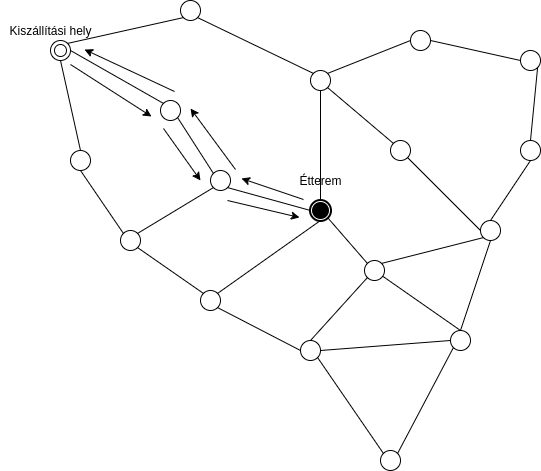
\includegraphics[scale=0.5]{images/Astar.png}

\Section{A probléma megoldása}

A* algoritmus

Az eljárásban a kiértékelő függvényünk a heurisztikus fügvény. Maga a fő ciklus minden iterációjánál az A*-nak meg kell határoznia az általala kiterjesztendő utat. A szakasz költségét és a célhoz érésnek költségét veszi figyelembe. Így az A* meghatározza az f(n) = g(n) + h (n) függvényt minimalizáló utat. n-nel jelölik a következő úton található csúcsot, ezáltal g(n) a kezdőpontból n-ig tartó út költsége. A heurisztikus függvényt h(n)-nel azonosítható, ez pedig nem más mint az n-től a célig vezető legolcsóbb út költését becsüli.
Az algoritmus legnagyobb hibája, hogy nem alkalmazható sok nagyméretű problémához nem praktikus, mivel a nagy memóriória igénye van, mert a meglátogatott csúcsokat eltárolja.

f(n) = g(n) + h (n) \\
g(n) - a kezdőpontból n-ig tartó út költsége \\
h(n) - n-től a célig vezető legolcsóbb út költése 

\Section{A megoldás implementálása}

\begin{python}

class Node():

    def __init__(self, parent=None, position=None):
        self.parent = parent
        self.position = position

        self.g = 0
        self.h = 0
        self.f = 0

    def __eq__(self, other):
        return self.position == other.position

def astar(maze, start, end):
    start_node = Node(None, start)
    start_node.g = start_node.h = start_node.f = 0
    end_node = Node(None, end)
    end_node.g = end_node.h = end_node.f = 0

    open_list = []
    closed_list = []

    open_list.append(start_node)

    while len(open_list) > 0:

        current_node = open_list[0]
        current_index = 0
        for index, item in enumerate(open_list):
            if item.f < current_node.f:
                current_node = item
                current_index = index

        open_list.pop(current_index)
        closed_list.append(current_node)

        if current_node == end_node:
            path = []
            current = current_node
            while current is not None:
                path.append(current.position)
                current = current.parent
            return path[::-1] # Return reversed path

        children = []
        for new_position in [(0, -1), (0, 1), (-1, 0), (1, 0), (-1, -1), (-1, 1), (1, -1), (1, 1)]: # Adjacent squares

            node_position = (current_node.position[0] + new_position[0], current_node.position[1] + new_position[1])

            if node_position[0] > (len(maze) - 1) or node_position[0] < 0 or node_position[1] > (len(maze[len(maze)-1]) -1) or node_position[1] < 0:
                continue

            new_node = Node(current_node, node_position)

            children.append(new_node)

        for child in children:

            for closed_child in closed_list:
                if child == closed_child:
                    continue

            child.g = current_node.g + 1
            child.h = ((child.position[0] - end_node.position[0]) ** 2) + ((child.position[1] - end_node.position[1]) ** 2)
            child.f = child.g + child.h

            for open_node in open_list:
                if child == open_node and child.g > open_node.g:
                    continue

            open_list.append(child)


def main():

    maze = [[0, 0, 0, 0, 0, 0, 0, 0, 0, 0],
            [0, 0, 0, 0, 0, 0, 0, 0, 0, 0],
            [0, 0, 0, 0, 0, 0, 0, 0, 0, 0],
            [0, 0, 0, 0, 0, 0, 0, 0, 0, 0],
            [0, 0, 0, 0, 0, 0, 0, 0, 0, 0],
            [0, 0, 0, 0, 0, 0, 0, 0, 0, 0],
            [0, 0, 0, 0, 0, 0, 0, 0, 0, 0],
            [0, 0, 0, 0, 0, 0, 0, 0, 0, 0],
            [0, 0, 0, 0, 0, 0, 0, 0, 0, 0],
            [0, 0, 0, 0, 0, 0, 0, 0, 0, 0]]

    start = (0, 0)
    end = (7, 6)

    path = astar(maze, start, end)
    print(path)


if __name__ == '__main__':
    main()

\end{python}

\Section{A megoldás tesztelése}


